\documentclass[12pt]{article}
\usepackage[fleqn]{amsmath}
\usepackage[document]{ragged2e}
\usepackage{amsfonts}
\usepackage{amssymb}
\usepackage{setspace}
\usepackage{textcomp}
\doublespacing
\usepackage{amsthm}
\theoremstyle{definition}
\newtheorem{definition}{Definition}[section]
\usepackage{graphicx}
\graphicspath{ {plots/} }
\usepackage[margin=3cm]{geometry}
\usepackage{caption}
\usepackage{subcaption}


\title{Parameter Estimation for Infinite L\'{e}vy Processes via Sequential Monte Carlo}
\author{Liew Kuang Chen Joel}
\begin{document}
\maketitle
\newpage 
\section*{Acknowledgements}
\newpage
\section*{Abstract}
\newpage

\tableofcontents
\newpage

\section{Introduction}

\section{Preliminaries}

\subsection{The L\'{e}vy Process}
In this paper, we will be using the Variance Gamma model from the family of Infinite Activity L\'{e}vy Processes. For the uninitiated, we will first go through the basics.
\theoremstyle{definition}
\begin{definition}{L\'{e}vy Process}\\
A L\'{e}vy Process, $X_{t}$, is a cadlag stochastic process on $(\Omega,\mathcal{F}_{t},P)$,with $X_{0}=0$ and has the following properties:\\
1. Independent increments: $X_{t+j+1} - X_{t+j} \perp X_{t+k+1} - X_{t+k}, \forall k,j \ge 0 , k \neq j$\\
2. Stationary increments: The Law of $X_{t+h} - X_{t}$ does not change for any $t$.\\
3. Stochastic continuity: For any $\epsilon>0, \lim_{h\rightarrow 0} P(|X_{t+h}-X_{t}|>\epsilon) = 0$
\end{definition}
\justify The L\'{e}vy Process also satisfies the Infinite Divisibility property.
\begin{definition}{Infinite Divisibility} \\
For $n\ge 2$, a probability distribution F is infinitely divisibile if there exists $n$ i.i.d. random variables $Y_{1},Y_{2},...$ such that $\sum_{i=1}^{n} Y_{i}$ has distribution F.
\end{definition}
\justify One common distribution satisfying the infinite divisibility condition is the Normal Distribution. If $X \sim N(\mu,\sigma^{2})$, then $X = \sum_{i=1}^{n} Y_{i}$,where $Y_{i} \sim N(\frac{\mu}{n},\frac{\sigma^{2}}{n})$.

\justify Due to fact that L\'{e}vy Processes are semimartingales and that their increments are independent, the process is Markovian and therefore in line with the Efficient Market Hypothesis. Hence, such processes are suitable to model asset prices (Li 2006). 
\subsubsection{Infinite Activity Processes - Variance Gamma}
The probability densities of most L\'{e}vy processes are not known in closed forms. However, their characteristics function $\phi_{X_{t}}(u)$ is as follows:
\begin{center}
$
\phi_{X_{t}}(u) = E[\exp^{iuX_{t}}] = \exp^{-t\psi_{x}(u)},t\ge 0
$
\end{center}


\justify where $\psi_{x}(u)$ is the characteristic exponent of $X$ (Tankov) and satisfies the follow L\'{e}vy-Khintchine formula
\begin{center}
$\psi_{x}\equiv -i\mu u + \frac{\sigma^{2}u^{2}}{2} + \int_{R_{0}} (1-\exp^{iux}+iux1_{|x|<1})\pi (dx) $\\
where $R_{0} = R$ \textbackslash $\{0\}$ and $\pi$ is a $R_{0}$ Radon measure and \\
$\int_{R_{0}} |x|^{2} \pi (dx)< \infty \qquad \int_{R_{0}} \pi (dx) < \infty$
\end{center}

Unlike the Finite Activity models (such as the Merton Jump Model) under the family of L\'{e}vy Processes, the infinite-activity models allow infinite jumps within a finite time interval. Hence,
\begin{center}
$\int_{R_{0}} \pi (dx) \not< \infty$
\end{center}

Within the category of Infinite Activity L\'{e}vy Processes, the jump process can have either finite or infinite variation. In the case of the finite/infinite variation, the sum of the absolute distance is finite/infinite over any finite time interval. For this paper, we will only be focussing on the Variance Gamma Process - a member from the Infinite Activity with Finite Variation. This process, $Z_{t}$, is created using a Brownian Motion, $B_{t}$, with drift $\gamma$ and variance $\sigma_{j}^2$, subordinated by an independent gamma process, $G_{t}$, with parameter $\alpha$.
\begin{center}
$dZ_{t} = \gamma dG_{t} + \sigma_{j}\sqrt{dG_{t}}dB_{t}$\\
$G_{t+t_{0}} - G_{t} \sim Ga(\frac{t}{\alpha},\frac{1}{\alpha})$
\end{center}
with the L\'{e}vy measure given by
\begin{center}
$\pi(dx) = \frac{A^{2}_{\pm}\exp(-\frac{A_{\pm}}{B_{\pm}}|x|)}{B_{\pm}|x|}(dx)$
\end{center}
where $A_{\pm}=\frac{1}{v}\sqrt{\frac{\gamma^{2}v^{2}}{4}+\frac{\sigma^{2}}{2} \pm \frac{\gamma v}{2}},B_{\pm}=A^{2}_{\pm}v$. In the case where $\gamma=0$, the jumps are symmetric about 0.

\subsection{Sequential Monte Carlo}
\subsubsection{Perfect Monte Carlo}
Suppose we are able to simulate $N$ i.i.d. random samples/particles $\{\theta_{0:t}^{i},i=1,2,...,N\}$ from a particular distribution (which in this paper, we are refering to the posterior distribution) - $p(\theta_{0:t}|y_{0:t})$. Then, the empirical estimate of this distribution is
\begin{equation}
	\begin{aligned}
		P_{N}(d\theta_{0:t}|y_{0:t}) = \frac{1}{N}\sum_{i=1}^{N}\delta_{\theta_{0:t}^{i}}(d\theta_{0:t})
	\end{aligned}
\end{equation}
where $\delta_{\theta_{0:t}^{i}}(d\theta_{0:t})$ refers to the delta-dirac mass located at $\theta_{0:t}^{i}$. One can then obtain the estimate of $E[f(\theta_{0:t})]$ via
\begin{equation}
	\begin{aligned}
		E[f(\theta_{0:t})]_{est} = \int f(\theta_{0:t}^{i}) \,P_{N}(d\theta_{0:t}|y_{0:t}) = \frac{1}{N}\sum_{i=1}^{N}f(\theta_{0:t}^{i})
	\end{aligned}
\end{equation}
If the posterior variance of $f(\theta_{0:t})$ satisfies \(\sigma^{2} :=\) $E[f(\theta_{0:t})^{2}] - E[f(\theta_{0:t})]^{2} < + \infty $, 
\begin{equation}
	\begin{aligned}
		var(E[f(\theta_{0:t})]_{est}) = \frac{\sigma^{2}}{N}
	\end{aligned}
\end{equation}
and by the Strong Law of Large Numbers,
\begin{equation}
	\begin{aligned}
		E[f(\theta_{0:t})]_{est} \mathrel{\mathop{\rightarrow}^{\mathrm{a.s.}}_{N \rightarrow \infty}} E[f(\theta_{0:t})]
	\end{aligned}
\end{equation}
Also, if $\sigma^{2} < +\infty$, the Central Limit Theorem holds
\begin{equation}
	\begin{aligned}
		\sqrt{N}(E[f(\theta_{0:t})]_{est} - E[f(\theta_{0:t})]) \mathrel{\mathop{\Longrightarrow}_{N \rightarrow \infty}} N(0,\sigma^{2})]
	\end{aligned}
\end{equation}
Unfortunately, it often is difficult to sample from the posterior distribution, especially in high dimensional cases. Markov Chain Monte Carlo (MCMC) methods is a possible alternative, but are unsuited for recursive problems. Hence, we will introduce a new method in this paper.
\subsubsection{Importance Sampling}
One classical method is the use of Importance Sampling method (Geweke 1989). Suppose we are interested in evaluating $E[f(\theta_{0:t})]$. Using a proposal density $\pi(\theta_{0:t}|y_{0:t})$, from which we can easily sample from, we get the following:
\begin{equation}
	\begin{aligned}
		E[f(\theta_{0:t})]_{est} &= \int f(\theta_{0:t}^{i}) \,P_{N}(d\theta_{0:t}|y_{0:t}) \\
		&= \int f(\theta_{0:t}^{i})p(\theta_{0:t}|y_{0:t}) \,d\theta_{0:t} \\
		&= \int f(\theta_{0:t}^{i})\frac{p(\theta_{0:t}|y_{0:t})}{\pi(\theta_{0:t}|y_{0:t})}\pi(\theta_{0:t}|y_{0:t})\,d\theta_{0:t} \\
		&= \int f(\theta_{0:t}^{i})w(\theta_{0:t}^{i})\pi(\theta_{0:t}|y_{0:t})\,d\theta_{0:t} \\
	\end{aligned}
\end{equation}
Since we can easily simulate from $N$ i.i.d. from $\pi(\theta_{0:t}|y_{0:t})$, we can get an estimate of $E[f(\theta_{0:t})]$
\begin{equation}
	\begin{aligned}
		\hat{E}[f(\theta_{0:t})]_{est} &= \int f(\theta_{0:t}^{i})\,\hat{P}(d\theta_{0:t}) \\
		&=\frac{\frac{1}{N}\sum_{i=1}^{N}f(\theta_{0:t}^{i})w(\theta_{0:t}^{i})}{\frac{1}{N}\sum_{i=1}^{N}w(\theta_{0:t}^{i})} \\
		&= \sum_{i=1}^{N}f(\theta_{0:t}^{i})W(\theta_{0:t}^{i}) \\
	\end{aligned}
\end{equation}
where $w(\theta_{0:t}^{i})$ and $W(\theta_{0:t}^{i})$ is known as the importance weights and normalised weights respectively. Note that we are now operating under the new measure 
\begin{equation}
	\begin{aligned}
		\hat{P}(\theta_{0:t}) = \frac{1}{N}\sum_{i=1}^{N}\delta_{\theta_{0:t}^{i}}(d\theta_{0:t})W(\theta_{0:t}^{i})
	\end{aligned}
\end{equation}
The Importance Sampling method does not work well in this form (especially in high dimensional cases). In addition, under $\mathcal{F}_{t+1}$, one has to recompute the weights/normalised weights despite having the weights/normalised weights at $\mathcal{F}_{t}$ - the recursive problem has yet to be solved! However, this has spawned new innovations, one which we will discuss and use in this paper.
\subsubsection{Sequential Importance Sampling (SIS)}
The Importance Sampling Method can be improved to include new information, $\mathcal{F}_{t+1}$, without recomputing $\{\theta_{0:t}^{i},i=1,2,...,N\}$. Using the following fact,
\begin{equation}
	\begin{aligned}
		P(A_{n},..,A_{1}|B) = P(A_{n}|A_{n-1},..,B)P(A_{n-1}|A_{n-2},..,B)..P(A_{1}|B)
	\end{aligned}
\end{equation}
we get,
\begin{equation}
	\begin{aligned}
		\pi(\theta_{0:t+1}|y_{1:t+1}) = \pi(\theta_{t+1}|\theta_{0:t},y_{1:t+1})\pi(\theta_{0:t}|y_{1:t})
	\end{aligned}
\end{equation}
After iterating,
\begin{equation}
	\begin{aligned}
		\pi(\theta_{0:t+1}|y_{1:t+1}) = \pi(\theta_{0})\prod_{i=1}^{t+1}\pi(\theta_{i}|\theta_{0:i-1},y_{1:i})
	\end{aligned}
\end{equation}
Our weights can then be recursively updated using the following
\begin{equation}
	\begin{aligned}
		W(\theta_{0:t+1}^{i}) \propto W(\theta_{0:t}^{i}) \frac{p(y_{t+1}|\theta_{t+1}^{i})p(\theta_{t+1}^{i}|\theta_{t}^{i})}{\pi(\theta_{t+1}^{i}|\theta_{0:t}^{i},y_{1:t+1})}
	\end{aligned}
\end{equation}
One importance case (which we will use) is when we adopt the prior distribution as the importance distribution at $t=0$. However, one drawback of using the SIS method is that one is unable to get the Importance distribution $\pi_{t}(\theta_{1:t})$
\begin{equation}
	\begin{aligned}
		\pi_{t}(\theta_{1:t}) = \int \pi_{1}(\theta_{1})\prod_{k=2}^{t}K_{k}(\theta_{k-1},\theta_{k}) \,d\theta_{1:t-1}
	\end{aligned}
\end{equation}
Although there are some approximations by used for local random-walk moves, the complexity of the algorithm is $O(N^2)$ and one cannot compute $K_{t}(\theta_{t-1},\theta_{t})$ pointwise (Del Moral, Doucet, Jasra 2006).
\subsubsection{Sequential Monte Carlo Samplers (SMC)}
The main idea of the Sequential Monte Carlo Samplers is to introduce artificial backward Markov Kernels, $L_{t-1}$ and propose an auxiliary variable technique. Given
\begin{center}
$\widetilde{p_{t}}(\theta_{1:t}) = \frac{\widetilde{\gamma_{t}}(\theta_{1:t})}{C_{t}}$\\
$\widetilde{\gamma_{t}}(\theta_{1:t}) = \gamma_{t}(\theta_{t})\prod_{k=1}^{t-1} L_{k}(\theta_{k+1},\theta_{k})$
\end{center}
where $C_{t}$ is the normalisation constant for the unnormalised probability density $\widetilde{\gamma_{t}}(\theta_{1:t})$ and $\gamma_{t}(\theta_{t})$ is the actual unnormalised probability density function of the distribution in question. Suppose, at $\mathcal{F}_{t}$, we have $\{W^{i}_{t},\theta_{0:t}^{i},i=1,2,...,N\}$ approximating $\widetilde{p_{t}}(\theta_{1:t})$
\begin{center}
$\widetilde{p_{t}^{N}}(d\theta_{1:t})=\sum_{i=1}^{N} W^{i}_{t} \delta_{\theta_{1:t}}(d\theta_{1:t})$\\
$W^{i}_{t}(\theta^{i}_{1:t}) = \frac{w^{i}_{t}(\theta^{i}_{1:t})}{\sum_{i=1}^{N} w^{i}_{t}(\theta^{i}_{1:t})}$
\end{center}
where $w_{t}^{i}(\theta_{1:t}^{i})$ is the standard Importance weights in (7). Now, at $\mathcal{F}_{t+1}$, we bring the particles forwards via the Markov Kernel $K_{t+1}(\theta_{t},\theta_{t+1})$. The unnormalised weights is computed using
\begin{equation}
w^{i}_{t+1}(\theta_{1:t+1}) = \frac{\gamma_{t+1}(\theta_{1:t+1})}{\pi_{t+1}(\theta_{1:t+1})} = w^{i}_{t}(\theta_{1:t})\widetilde{w}^{i}_{t+1}(\theta_{t},\theta_{t+1})
\end{equation}
where the incremental weight, $\widetilde{w}^{i}_{t+1}(\theta_{t},\theta_{t+1})$ equals to
\begin{equation}
\widetilde{w}^{i}_{t+1}(\theta_{t},\theta_{t+1}) = \frac{\gamma_{t+1}(\theta_{t+1})L_{t}(\theta_{t+1},\theta_{t})}{\gamma_{t}(\theta_{t})K_{t+1}(\theta_{t},\theta_{t+1})}
\end{equation}
In the case of Markov Chain Monte Carlo Kernels, we can define the backward Markov Kernel suboptimally, by
\begin{equation}
L_{t}(\theta_{t+1},\theta_{t}) = \frac{p_{t+1}(\theta_{t})K_{t+1}(\theta_{t},\theta_{t+1})}{p_{t+1}(\theta_{t})}
\end{equation}
If $p_{t} \approx p_{t+1}$, then
\begin{center}
$L_{t}(\theta_{t+1},\theta_{t})  \approx L^{sub}_{t}(\theta_{t+1},\theta_{t})  = \frac{p_{t}(\theta_{t})K_{t+1}(\theta_{t},\theta_{t+1})}{\int p_{t}(\theta_{t})K(\theta_{t},\theta_{t+1})\,d\theta_{t}}$
\end{center}
Thus, we will have the following incremental weights
\begin{equation}
\widetilde{w}_{t+1}^{i}(\theta_{t},\theta_{t+1}) = \frac{\gamma_{t+1}(\theta_{t})}{\gamma_{t}(\theta_{t})}
\end{equation}

\section{Literature Review}
\subsection{The Model}
For the purposes of this paper, we will be focusing on the Stochastic Volatility with Variance Gamma Jumps in Returns (SVVG). The model is as follows:

\begin{equation}
	\begin{aligned}
		dY_{t} &=\mu dt+\sqrt{v_{t}}[\rho dW_{1t}+\sqrt{1-\rho ^{2}} dW_{2t}] + dZ_{t} &\\
		dv_{t} &= \kappa (v - v_{t})dt+\sigma _{v}\sqrt{v_{t}}dW_{1t} &\\
		dZ_{t} &= \gamma dG_{t} + \sigma _{j} \sqrt{dG_{t}}dB_{t}
	\end{aligned}
\end{equation}
Using Euler Discretization, we have the following:
\begin{equation}
	\begin{aligned}
		Y_{t+1} &= Y_{t} + \mu\Delta + \sqrt{v_{t}\Delta}\epsilon_{t+1}^{y}+Z_{t+1}\\
		v_{t+1} &= v_{t} + \kappa(\upsilon - v_{t})\Delta + \sigma_{v}\sqrt{v_{t}\Delta}\epsilon_{t+1}^{v}\\
		Z_{t+1} &= \gamma G_{t+1} + \sigma_{j}\sqrt{G_{t+1}}\epsilon_{t+1}^{Z}
	\end{aligned}
\end{equation}
where both $\epsilon_{t+1}^{y}$ and $\epsilon_{t+1}^{v}$ follow $N(0,1)$ with $corr(\epsilon_{t+1}^{y},\epsilon_{t+1}^{v})=\rho$ while $\epsilon_{t+1}^{y},\epsilon_{t+1}^{v} \perp G_{t+1}$. The Jump Process $Z_{t+1}$ follows a variance gamma process where $\epsilon_{t+1}^{Z}$ follows $N(0,1)$ and $\epsilon_{t+1}^{Z} \perp \epsilon_{t+1}^{y},\epsilon_{t+1}^{v},G_{t+1}$. $G_{t+1}$ follows a Gamma Distribution, $\Gamma (\alpha,\beta)$.\\
Hence, we have observations $(Y_{t})_{t=0}^{T}$; latent variables $(v_{t})_{t=0}^{T},(Z_{t})_{t=1}^{T},(G_{t})_{t=1}^{T}$; and parameters $\Theta = \{\mu,\rho,\kappa,\upsilon,\sigma_{v},\gamma,\sigma_{j}\}$. For convenience, we let $\theta = \{\Theta,(v_{t})_{t=0}^{T},(Z_{t})_{t=1}^{T},(G_{t})_{t=1}^{T} \}$.
\subsection{Derivation of Posterior Density}
Since $corr(\epsilon_{t+1}^{y},\epsilon_{t+1}^{v})=\rho$ and $\epsilon_{t+1}^{y},\epsilon_{t+1}^{v} \sim N(0,1)$, conditioning on the values of $Z_{t+1}$,$v_{t}$ and $\Theta$, we get
\begin{equation}
	\begin{aligned}
\begin{pmatrix}
Y_{t+1} - Y_{t}\\
v_{t+1} - v_{t}
\end{pmatrix} | v_{t},Z_{t+1},\Theta
\sim
N
\begin{pmatrix}
\begin{pmatrix}
\mu \Delta + Z_{t+1} \\
\kappa (\theta - \upsilon) \Delta \\
\end{pmatrix}
,
v_{t} \Delta
\begin{pmatrix}
1 & \rho \sigma_{v} \\
\rho \sigma_{v} & \sigma_{v}^2 \\
\end{pmatrix}
\end{pmatrix}
	\end{aligned}
\end{equation}
As for the variance gamma process, Li et. al (2006) shows that conditioning on $G_{t+1}$ and $\Theta$, we get \\
\begin{center}
$J_{t+1} | G_{t+1},\Theta \sim N(\gamma G_{t+1},\sigma_{j}^{2}G_{t+1})$ \\
$G_{t+1} | \Theta \sim \Gamma(\frac{\Delta}{v},v)$\\
\end{center}
However, in Jasra (2011), it is shown that $G_{t+1}$ can be integrated out:
\begin{equation}
	\begin{aligned}
		p(Z_{t+1}|\Theta) &= \int p(Z_{t+1}|G_{t+1},\Theta)p(G_{t+1}|\Theta) \,dG_{t+1}\\
		&= \frac{2exp(\frac{\gamma Z_{t+1}^{2}}{\sigma})}{\alpha^{\frac{t-u}{\alpha}}\sqrt{2\pi} \Gamma(\frac{t-u}{\alpha},\frac{1}{\alpha})}\Bigg(\frac{Z_{t+1}^{2}}{\gamma^{2}+2\frac{\sigma^{2}}{\alpha}}\Bigg)^{\frac{t-u}{2\alpha}-\frac{1}{4}}K_{\frac{t-u}{\alpha}-\frac{1}{2}}\Bigg(\frac{\sqrt{Z_{t+1}^{2}(\gamma^{2}+\frac{2\sigma^{2}}{\alpha})}}{\sigma^{2}}\Bigg)
	\end{aligned}
\end{equation}
where $K_{a}(.)$ is the modified Bessel Function of the second kind, and $\sigma = \sigma_{j}\sqrt{t-u}$. In this paper, we will let $\alpha = t-u$. Thus, the simulation procedure is reduced by one dimension, and this reduces the simulation complexity, since there is one lesser latent variable to udpate. \\
As for the priors, we will follow the ones subscribed by Li (2006).\\
\\
$p(\Theta)=p(\mu)p(\gamma)p(\sigma_{j})p(\kappa)p(\sigma_v,\rho)p(\upsilon)$\\
$\mu,\gamma,\sigma_{j} \sim N(0,1)$\\
$\kappa,\upsilon \sim N(0,1)$ truncated at 0\\
Reparameterize $(\rho,\sigma_{v})$ to $(\phi,w)$, where $\phi = \sigma_{v} \rho , w = \sigma_{v}^{2}(1-\rho^{2})$\\
$w \sim IG(1.0,0.5), \phi | w ~ N(0,0.5w)$\\

\noindent Now, the posterior distribution is as follows:
\begin{equation}
\begin{aligned}
p(\Theta,v_{1:n},Z_{1:n}|Y_{0:n}) \propto p(\Theta) \prod_{i=0}^{n} p(Y_{i+1},v_{i+1}|Y_{i},v_{i},Z_{i+1},\Theta)p(Z_{i+1}|\Theta)
\end{aligned}
\end{equation}

\subsection{Simulation using a Sequence of Densities}
Using the following densities,
\begin{equation}
	\begin{aligned}
		\pi_{k}(\theta_{1:n}|y_{0:n}) \propto p(\Theta)\prod_{i=1}^{n}[p(y_{i},v_{i}|y_{i-1},v_{i-1},z_{i},\Theta)^{\zeta_{k}}p(z_{i}|\Theta)] 
	\end{aligned}
\end{equation}
where $0\leqslant\zeta_{1}<...<\zeta_{p}=1.$ 
\noindent The idea is to simulate from an 'easy' density, before shifting the particles to a much more difficult density. At $\zeta_{1}$, the tempered posterior density focusses more on the priors than when compared to $\zeta_{k}$ where $k>1$. Overtime, as the algorithm iterates, the tempered posterior focusses less on the prior and more on the liklihood. Hence, when $\zeta_{p}=1$, the particles now exist in the target posterior density.

\subsection{Simulation Procedure}
To start off the simulation, we first sample from the prior distribution $\pi_{0}$ and Importance sampling is then conducted as below
\begin{equation}
	\begin{aligned}
		w_{1}(\theta^{i}) &= \frac{\pi_{1}(\theta_{1}^{i}|y_{0:n})}{\pi_{0}(\theta_{1}^{i}|y_{0:n})} \\
		W_{1}(\theta^{i}) &= \frac{w_{1}^{i}}{\sum_{i=1}^{M} w_{1}^{i}}
	\end{aligned}
\end{equation}
At the second iteration, the particles are shifted from $\pi_{1}$ to $\pi_{2}$ via a kernel of invariant distribution $P_{2}(\theta_{1}^{i},\theta_{2}^{i})$
\begin{equation}
	\begin{aligned}
		w_{2}(\theta^{i}) &= \frac{\pi_{2}(\theta_{2}^{i}|y_{0:n})}{\int \pi_{1}(\theta_{1}^{i}|y_{0:n})P(\theta_{1}^{i},\theta_{2}^{i}) \,d\theta_{1}}
	\end{aligned}
\end{equation}
There are many choices of kernels, but in this paper we will adopt the Random Walk Metropolis Kernel. Hence, for $t\geqslant2$,
\begin{equation}
	\begin{aligned}
		w_{k}(\theta^{i}) &= W_{k-1}^{i}(\theta^{i})\prod_{i=1}^{n} p(y_{i}|y_{i-1},v_{i},z_{i},\Theta)^{\zeta_{k}-\zeta_{k-1}}
	\end{aligned}
\end{equation}

\noindent For the Random Walk Metropolis Kernel, one has to specify the proposal variance $\psi_{k+1}$ in order for one to update the parameter values. Using adaptive MCMC techniques (Andrieu, Moulines 2006), we approximate the mean and therefore the variance of the parameters at iteration $k$, for the next iteration $k+1$. Also, if the acceptance rate of the parameter is above $0.85$, we tune up the variability by a factor of 5. Likewise, if the acceptance rate of the parameter is below $0.15$, we tune down the variability by a factor of 1/5. 

\subsection{Resampling}
Like the problem encountered in the Sequential Importance Sampling, the variability of the weights increases as the iteration increases. This is termed as weight degeneracy (Doucet et. al 2001). Hence, to counter this problem, we resample the particles according to the normalised weights within the cloud of particles. After resampling, the weights of the particles are reset to 1. In this paper, we will be using the Multinomial Resampling method, even though more sophisticated methods exist. One point to note is that the resampling should occur too often. When resampling occurs, the number of unique particles fall, hence reducing the particles' approximation of the target density. One criterion to measure the variability of the weights is the Effective Sample Size (ESS) (Doucet et al. 2001). 
\begin{equation}
	\begin{aligned}
		ESS_{k} = \frac{(\sum_{i=1}^{M} w_{k}^{i})^{2}}{\sum_{i=1}^{M} (w_{k}^{i})^{2}}=
		\frac{(\sum_{i=1}^{M} W_{k}^{i} \prod_{i=1}^{n} p(y_{i}|y_{i-1},v_{i},z_{i},\Theta)^{\zeta_{k}-\zeta_{k-1}})^{2}}{\sum_{i=1}^{M} (W_{k}^{i}\prod_{i=1}^{n} p(y_{i}|y_{i-1},v_{i},z_{i},\Theta)^{\zeta_{k}-\zeta_{k-1}})^{2}}
	\end{aligned}
\end{equation}
The idea of this criterion is to give insight on the approximate number of samples relative to an independent simulation approach (Jasra et. al 2006). When $ESS_{k}$ drops below some threshold $l$, we resample. \\
\\
\noindent In this paper, at iteration $k$ of the algorithm, we let $ESS_{k}=0.95ESS_{k-1}$. Using the bisection method, we are able to calculate $\zeta_{k}$ using (18). 

\subsection{The SMC Algorithm}
Therefore, the algorithm is as follows:
At iteration k=1, sample $\theta_{1}^{i} \sim \pi_{1}$ for $i=1,..,M$ and compute\\
\begin{center}
$w_{1}(\theta^{i}) = \frac{\pi_{1}(\theta_{1}^{i}|y_{0:n})}{\pi_{0}(\theta_{1}^{i}|y_{0:n})}$\\
$W_{1}(\theta^{i}) = \frac{w_{1}^{i}}{\sum_{i=1}^{M} w_{1}^{i}}$
\end{center}
If $ESS_{k} \leqslant l$, resample and set $W_{1}(\theta^{i}) = 1/M$. Set $\psi_{k+1}$ for each kernel. \\
\noindent At iteration $k=2,..,p$, set $\zeta_{k}$ and compute
\begin{center}
$w_{k}(\theta^{i}) = \frac{\pi_{1}(\theta_{1}^{i}|y_{0:n})}{\pi_{0}(\theta_{1}^{i}|y_{0:n})}$\\
$W_{k}(\theta^{i}) = \frac{w_{k}^{i}}{\sum_{i=1}^{M} w_{k}^{i}}$
\end{center}
If $ESS_{k} \leqslant l$, resample and set $W_{k}(\theta^{i}) = 1/M$. If $k < l$, set $\psi_{k+1}$ for each kernel.
\section{Empirical Results}

\subsection{Simulation Tests}
We now provide evidence that this SMC algorithm can accurately estimate the parameters of the SVVG Model. First, using the SVVG Model, we generate 100 paths of 150 days of daily data. The initial value of the volatility is chosen to be 1 and the rest of the latent variables are randomly chosen within their ranges. Then, we run the SMC algorithm over these 100 paths to get us the posterior means of the parameters. The 100 different posterior parameter means are then used to generate the posterior densities of the parameter. The 95\% highest posterior density interval is also calculated.  \\
\begin{figure}
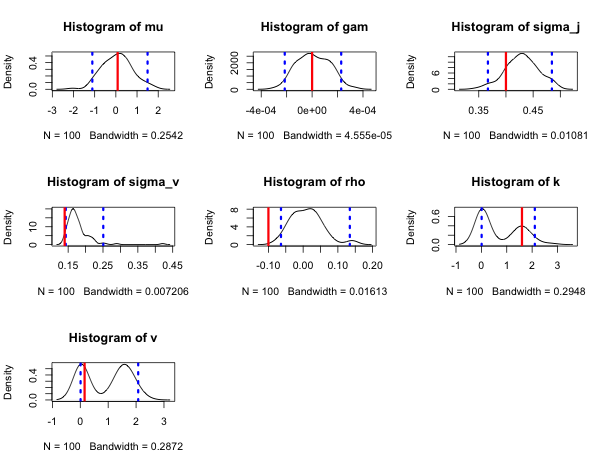
\includegraphics[width=\textwidth]{density_plots}
\caption{95\% Credible Interval is denoted by the blue dotted line. True value of the parameter of the SVVG Model denoted by the red solid line.}
\end{figure}
\\
From Table 1, 3 out of the 7 parameters do not lie within the 95\% credible interval. This could be due to the choice of $\Delta$ in the Euler Discretization which would affect the accuracy of the posterior parameter estimates. For this simulation, $\Delta$ was chosen to be $1/250$ to represent the daily close. One can choose a smaller $\Delta$ at the cost of higher complexity for the latent variables as one has to simulate data points between $(t,t+\Delta t)$. Note that from Table 1 and Figure 1, this SMC algorithm has been able to estimate $\mu$  quite accurately - a feature which we will use for our proposed Trading Strategy.
\begin{table}
\centering
\begin{tabular}{|c c c c c|} 
 \hline
 Parameter & True & 0.025 & Median & 0.975 \\
 \hline
 $\mu$ & 0.085 & -1.1108 & 0.0595 &1.4978 \\
 $\gamma$ & 0.0 & -0.0002 & 0.0000 & 0.0002 \\
 $\sigma_{j}$ & 0.4 & 0.3668 & 0.4293 & 0.4845\\
 $\sigma_{v}$ & 0.14 & 0.1432 & 0.1693 &0.2508\\
 $\rho$ & -0.1 & -0.0638 & 0.0100 & 0.1344\\
 $\kappa$ & 1.6 & 0.0107 & 0.0479 & 2.1061\\
 $v$ & 0.155& 0.0109 & 1.2968 & 2.0762\\ 
 \hline
\end{tabular}
\caption{95\% Credible Interval and Median}
\label{table:1}
\end{table}
\subsection{The Trading Strategy}
For this section we will introduce a trading strategy with the help of the SMC Algorithm. We will be using the daily data of S\&P500 from 3/1/2007 to 4/3/2016. Then given a user defined lookback period, $n$, we take a rolling window of $n$ Closes until 4/3/2016. Next, for each window, we perform the SMC algorithm to get us the posterior mean of $\mu$, which is the posterior expectation of the log returns of the instrument. After that, we generate buy/sell signals if $\mu>\mu_{thres}/\mu<-\mu_{thres}$. For the trading strategy, we take $n=30$, $\mu=0$. Also, we assume that we can buy/sell S\&P500. 

\subsubsection{Naive Trading Strategy}

We model the trading strategy with zero transaction costs. The signal generated from the window of Closes is to be applied on the next day's Open. Assuming that we fully invest our capital into this strategy, we get the following equity curve (Fig 3). It is interesting to note that this naive strategy has execellent returns (about 300\% returns) for the first 3 years, before its performance started to stagnate between 250\% to 350\% returns. Out of the 2309 trading days, this strategy longed on 1143 days (49.5\%) and shorted on 1130 days (49.2\%). Note that the first 30 days did not yield any signal as the first window of 30 days was used to ascertain the direction for the next day. Plotting the signal against time (Fig 4), it is observed that the strategy flips direction every 3-5 days. This is a obvious sign that the strategy is trading too often, and perhaps the reason why this Naive strategy does not work after 2010.
\begin{figure}
\centering
\begin{minipage}{0.5\textwidth}
  \centering
  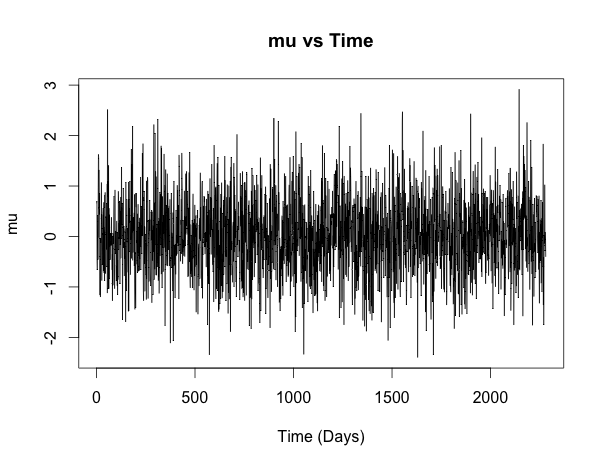
\includegraphics[width=1\textwidth]{ts1}
  \captionof{figure}{Plot of $\mu$ vs Time}
  \label{fig:test1}
\end{minipage}%
\begin{minipage}{0.5\textwidth}
  \centering
  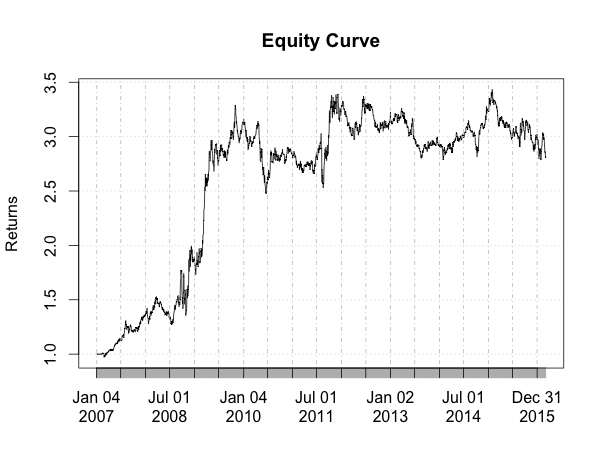
\includegraphics[width=1\textwidth]{ts2}
  \captionof{figure}{Plot of Equity vs TIme}
  \label{fig:test2}
\end{minipage}
\end{figure}

\begin{figure}
\centering
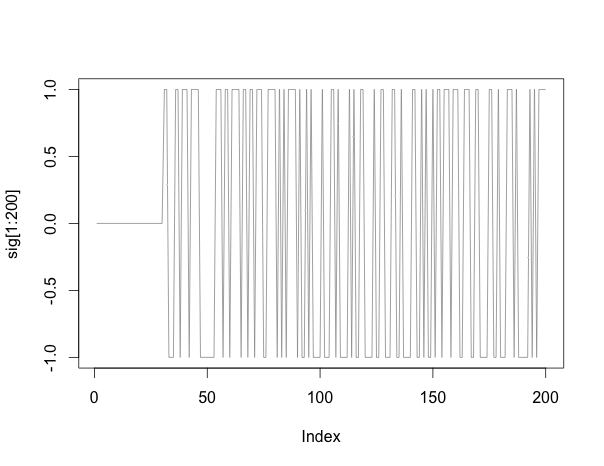
\includegraphics[width=0.5\textwidth]{ts3}
\caption{Position vs Time}
\end{figure}

\subsubsection{The Improved Strategy}
Now that we know that this strategy flip flops too often, we can consider adding a trailing stop for the strategy. Hence, the position remains until the trailing stop gets trigerred. For example, if we are long, the position remains until the low of the day gets below our trailing stop. Otherwise, as we ride the momentum up, the trailing stop increases. Mathematically, at day $t$, $TS_{buy,t} = max\{TS_{buy,t-1},Low_{t-l}\}$, where $l$ is a user defined lookback period and $Low_{t-l}$ denotes the Low of the instrument $l$ days ago. If we get stopped out of our position, we will re-enter the next day, assuming there is a signal to enter. For this toy example, we take $l=3$, transaction cost to be 0.5\% of total value of instrument bought/sold, value of each point of S\&P500 to be \$5 and the risk each trade to be 2\%. Our starting equity will be \$10,000.
\begin{figure}[ht]
\centering
\begin{minipage}{0.45\textwidth}
  \centering
  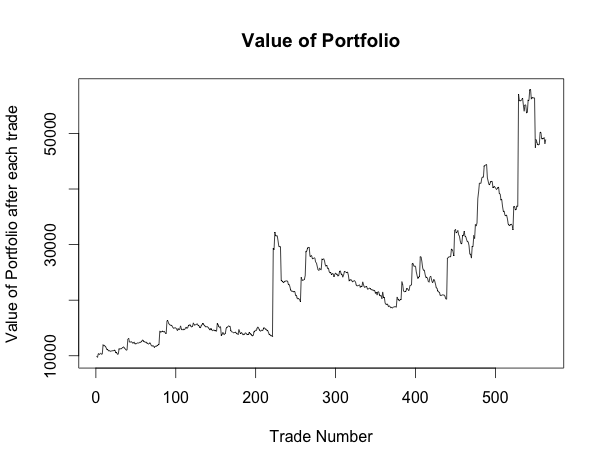
\includegraphics[width=1\textwidth]{ts4}
  \captionof{figure}{Plot of Portfolio vs Trade Number}
  \label{fig:test3}
\end{minipage}
\begin{minipage}{0.45\textwidth}
  \centering
  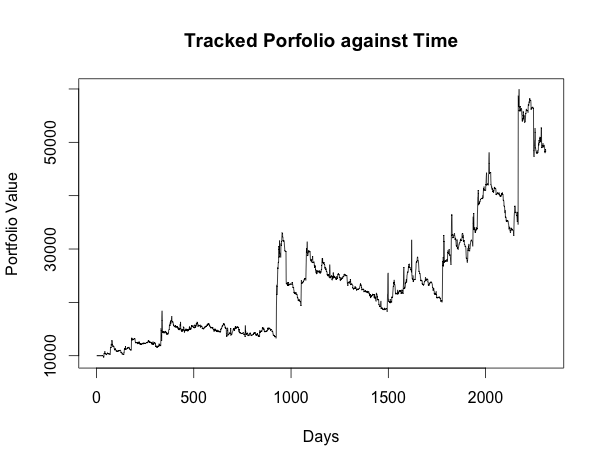
\includegraphics[width=1\textwidth]{ts5}
  \captionof{figure}{Plot of Portfolio vs TIme}
  \label{fig:test4}
\end{minipage}
\end{figure}\\
This improved strategy gives much better returns (500\% over 9 years) as compared to the Naive strategy. However, much can still be done for this strategy. For example, we can take do cross validation to optimise the lookback period for the trailing stop ($l$) and Close window ($n$). Also, we can add in fixed take profit points to see how this strategy performs. Despite the lucrative returns, this strategy is still considered unfavourable due to the long drawdown periods and volatility in its returns.

\begin{table}[ht]
\centering
\begin{tabular}{|c| c |c|} 
 \hline
 &Long & Short \\
 \hline
 Min. Return& -2.52\%& -3.86\%\\
1st Quantile Return& -1.24\% & -1.64\%\\
 Median Return& 0.0928\% & 0.0215\% \\
  Mean Return& 0.945\% & 0.554\% \\
 3rd Quantile Return & 0.711\% & 0.474\%\\
 Max. Return& 121.2\% & 64.9\%\\
 Success Rate& 56.4\% & 50.6\% \\ 
 \hline
\end{tabular}
\caption{Trade Statistics}
\label{table:2}
\end{table}
\subsubsection{The Optimized Strategy}
Now we see that this strategy has the potential to become a possible trading strategy, we will try to optimise the paramters using the training set and see what return we can generate over the 9 years. For our training set, we will be using the first 2 years (2007-2009) ie 500 readings. The metric we will be using to validate the strategy is called the CAR/MDD. It is simply the compounded annual return (CAR) divided by the max drawdown (MDD). Intuitively, a higher score means that our equity curve is smoother and therefore a better system.\\
We now include a form of market filter to prune out unfavourable entries. One logical extension of such is to buy/sell when the market drops/rises given that our posterior mean is positive/negative. Intuitively, this means that there is some sort of 'arbitrage' opportunity as the market has yet to price in the posterior expection of $\mu$. Due to the even distribution as seen in Table 3, we choose a threshold $r_{thres}=0.5$ as the limiting return. Now, we have cut down our potential signals at most 30\% on each direction. Hence, for each $r_{t}>r_{thres}=0.5$ and $r_{t}<-r_{thres}=-0.5$, we give a value of -1 and +1 respectively. We then take the rolling window of $l_{r}=5$ readings and give a buy and sell signal if the sum is greater than $S$ and lesser than $-S$ respectively(For the initial example we let $S=1$, and we will later optimise $S$ nad $l_{r}$). Like the improved trading strategy, we apply the same trailing stop. However, due to the fact we are now trading against the current direction of the market, we let initiate $TS_{buy,t} = min\{Open_{t}-(Hi_{t-1}-Low_{t-1}),Low_{t-l}\}$ and then trail accordingly. Combining the signal from the posterior $\mu$, we get the following equity curve (Fig 8) from the training set. We get a CAR/MDD = 1.960626 (MDD=14.10\%, CAR=27.64\%).
\begin{figure}
\centering
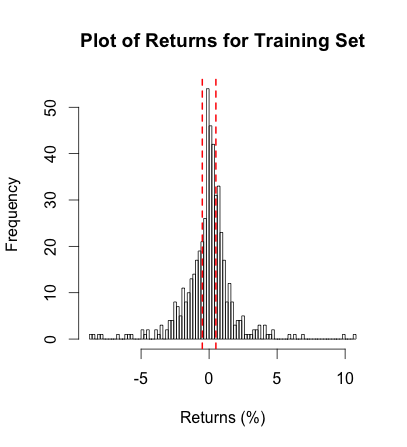
\includegraphics[width=0.5\textwidth]{returns}
\caption{Histogram of Returns of Training Set, with red lines indicating $\pm 0.5$}
\end{figure}
\begin{table}
\centering
\begin{tabular}{|c| c |c|} 
 \hline
$r_{t}<-0.5$ & $-0.5\le r_{t} \ge 0.5$ & $r_{t}>0.5$ \\
 \hline
30.2\% & 39.6\% & 30.2\% \\
 \hline
\end{tabular}
\caption{Empirical Distribution of Returns}
\label{table:3}
\end{table}

\begin{figure}
\centering
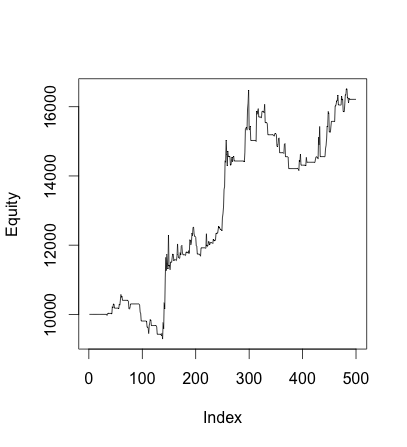
\includegraphics[width=0.5\textwidth]{trg}
\caption{Plot of Equity vs Time (Training Set)}
\end{figure}
From the contour plot, we look for the highest CAR/MDD with the flattest surrounding CAR/MDD, reason being that when we test out of sample, we do not want our CAR/MDD to fall too steeply. Hence, we ignore the point at (10,6). Instead, we take the point at (7,2), which gives us a CAR/MDD of 5.903.
\begin{figure}[ht]
\centering
\begin{minipage}{0.45\textwidth}
  \centering
  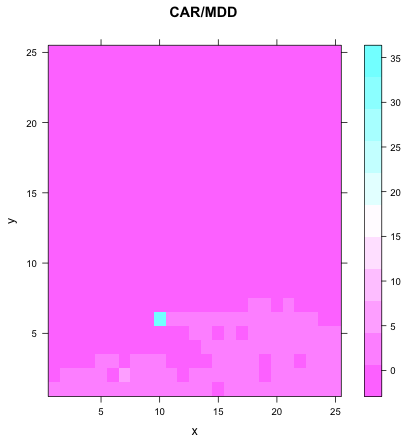
\includegraphics[width=1\textwidth]{opt_curve}
  \captionof{figure}{Optimization Contour Plot}
  \label{fig:test8}
\end{minipage}
\begin{minipage}{0.45\textwidth}
  \centering
  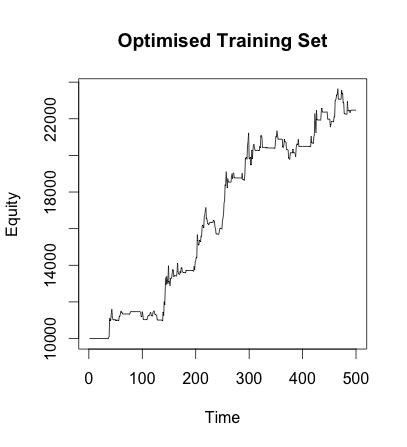
\includegraphics[width=1\textwidth]{opt_eq}
  \captionof{figure}{Plot of Portfolio vs Time (Opt)}
  \label{fig:test9}
\end{minipage}
\end{figure}\\
\begin{figure}[ht]
\centering
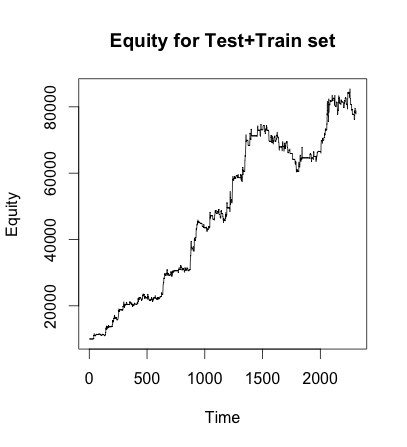
\includegraphics[scale=0.8]{final}
\captionof{figure}{Whole Equity Curve}
\label{fig:test9}
\end{figure}
Now, we seek to extend this signal to our test set and see how it unfolds. There is still quite a steep drawdown (Fig 11) of 19.26\%. Given the $l_{r}=7$ and $S=2$, we now choose to optimise the trailing stop loss lookback period ($l$)and the initial hard stop loss factor. The initial hard stop loss factor is the $SL_{fac}$ from $TS_{buy,t} = min\{Open_{t}-(Hi_{t-1}-Low_{t-1})*SL_{fac},Low_{t-l}\}$.Since we are now buying 'falling knives' (or selling rallies), the initial hard stop loss is required as $Low_{t-l}>Open_{t}$, which means that we do not have any reference point to put our trailing stop loss. During the optimization, we ignore points that give us a max drawdown of greater than 10\%. Our max point is at (8,1.4). We now have a very good equity curve with CAR/MDD = 7.45 (max drawdown = 8.75\% and annualised return = 65.29\%).
\begin{figure}[ht]
\centering
\begin{minipage}{0.45\textwidth}
  \centering
  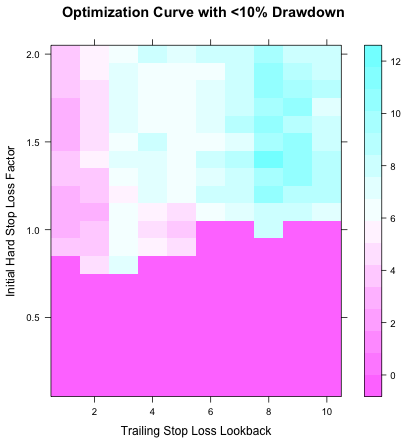
\includegraphics[width=1\textwidth]{opt2}
  \captionof{figure}{Optimization Contour Plot 2}
  \label{fig:test12}
\end{minipage}
\begin{minipage}{0.45\textwidth}
  \centering
  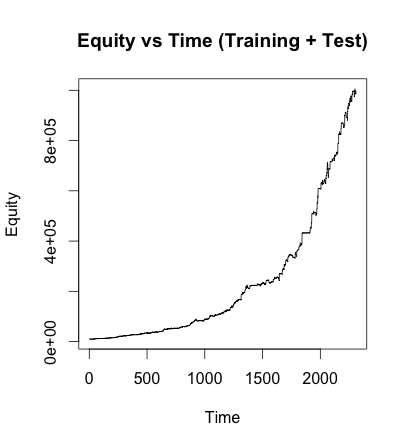
\includegraphics[width=1\textwidth]{opt2_eq}
  \captionof{figure}{Plot of Portfolio vs Time (Opt 2)}
  \label{fig:test13}
\end{minipage}
\end{figure}\\


\end{document}


